%============================================================
%  LEX v3.0 — Template Diagram ATD (Asas-Teori-Doktrin)
%  Perintah Copilot: /generate-viz ATD
%  Salin %============================================================
%  LEX v3.0 — Template Diagram ATD (Asas-Teori-Doktrin)
%  Perintah Copilot: /generate-viz ATD
%  Salin %============================================================
%  LEX v3.0 — Template Diagram ATD (Asas-Teori-Doktrin)
%  Perintah Copilot: /generate-viz ATD
%  Salin %============================================================
%  LEX v3.0 — Template Diagram ATD (Asas-Teori-Doktrin)
%  Perintah Copilot: /generate-viz ATD
%  Salin \input{../templates/atd-diagram} ke artikel Anda
%============================================================

\documentclass[tikz,border=10pt]{standalone}
\usepackage{tikz}
\usetikzlibrary{shapes.geometric, arrows.meta, positioning, fit, backgrounds, shadows}

\begin{document}

%------------------------------------------------------------
%  DIAGRAM 1: Kerangka ATD — Analisis Kasus
%------------------------------------------------------------
\begin{tikzpicture}[
  node distance = 1.6cm,
  every node/.style = {font=\small},
  box/.style = {
    rectangle, rounded corners=4pt, minimum width=3.8cm, minimum height=1cm,
    align=center, draw, thick
  },
  norma/.style   = {box, fill=blue!15,   draw=blue!60},
  asas/.style    = {box, fill=green!15,  draw=green!60},
  teori/.style   = {box, fill=orange!15, draw=orange!60},
  doktrin/.style = {box, fill=purple!15, draw=purple!60},
  hasil/.style   = {
    rectangle, rounded corners=6pt, minimum width=8cm, minimum height=1.2cm,
    align=center, draw=red!70, thick, fill=red!10
  },
  arrow/.style   = {-Stealth, thick, gray}
]

% Baris atas: empat elemen ATD
\node[norma]   (N) {Norma Positif\\{\footnotesize (Pasal/UU/Putusan)}};
\node[asas]    (A) [right=1.2cm of N] {Asas Hukum\\{\footnotesize (Ratio Legis)}};
\node[teori]   (T) [right=1.2cm of A] {Teori Hukum\\{\footnotesize (Filosofis/Yuridis)}};
\node[doktrin] (D) [right=1.2cm of T] {Doktrin Hukum\\{\footnotesize (Pendapat Ahli)}};

% Simbol plus di antara node
\node at ($(N.east)!0.5!(A.west)$) {\textbf{+}};
\node at ($(A.east)!0.5!(T.west)$) {\textbf{+}};
\node at ($(T.east)!0.5!(D.west)$) {\textbf{+}};

% Kotak hasil di bawah
\node[hasil] (H) [below=2cm of $(N.south)!0.5!(D.south)$]
  {\textbf{Konstatasi / Analisis Kasus}\\
   {\footnotesize [Isi dengan temuan analisis hukum Anda]}};

% Panah dari masing-masing elemen ke hasil
\draw[arrow] (N.south) -- ++(0,-0.6) -| (H.north);
\draw[arrow] (A.south) -- ++(0,-0.6) -| (H.north);
\draw[arrow] (T.south) -- ++(0,-0.6) -| (H.north);
\draw[arrow] (D.south) -- ++(0,-0.6) -| (H.north);

% Label judul
\node[above=0.4cm of $(N.north)!0.5!(D.north)$, font=\bfseries]
  {Kerangka Analisis ATD — LEX v3.0};

\end{tikzpicture}

%------------------------------------------------------------
%  DIAGRAM 2: Alur Prosedur Hukum (Flowchart)
%  Ganti label sesuai prosedur yang Anda analisis
%------------------------------------------------------------
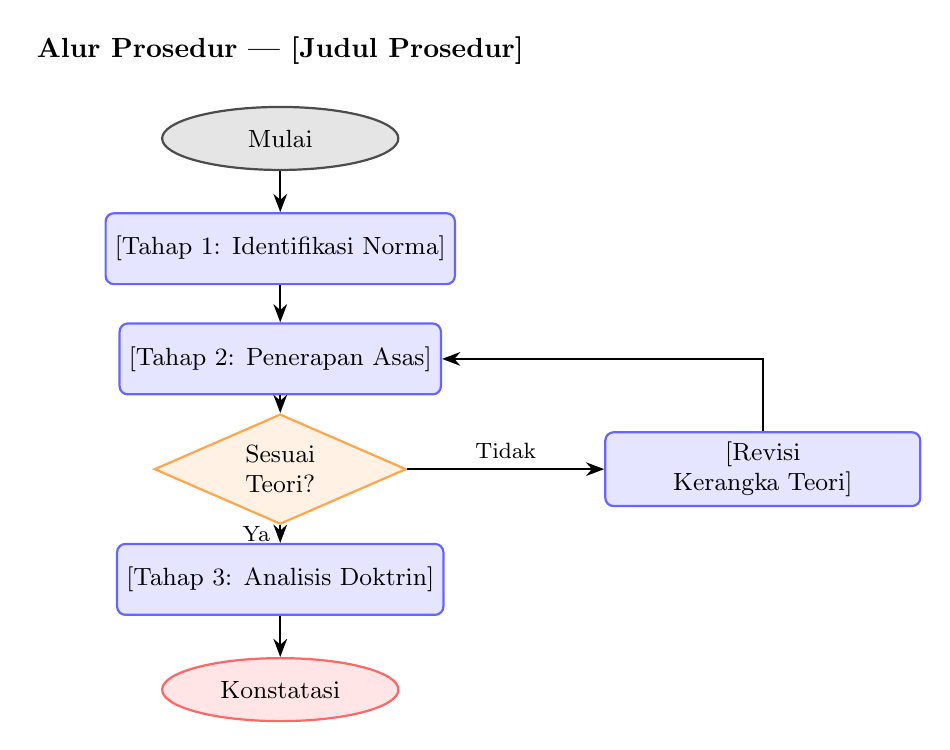
\begin{tikzpicture}[
  node distance=1.4cm,
  every node/.style={font=\small},
  start/.style={
    ellipse, draw=black!70, thick, fill=gray!20,
    minimum width=3cm, minimum height=0.8cm, align=center
  },
  proses/.style={
    rectangle, draw=blue!60, thick, fill=blue!10,
    minimum width=4cm, minimum height=0.9cm,
    rounded corners=3pt, align=center
  },
  keputusan/.style={
    diamond, draw=orange!70, thick, fill=orange!10,
    minimum width=3.2cm, minimum height=0.9cm,
    aspect=2, align=center
  },
  akhir/.style={
    ellipse, draw=red!60, thick, fill=red!10,
    minimum width=3cm, minimum height=0.8cm, align=center
  },
  arrow/.style={-Stealth, thick}
]

\node[start]     (mulai)   {Mulai};
\node[proses]    (p1)      [below of=mulai]   {[Tahap 1: Identifikasi Norma]};
\node[proses]    (p2)      [below of=p1]      {[Tahap 2: Penerapan Asas]};
\node[keputusan] (k1)      [below of=p2]      {Sesuai\\Teori?};
\node[proses]    (p3ya)    [below of=k1]      {[Tahap 3: Analisis Doktrin]};
\node[proses]    (p3tidak) [right=2.5cm of k1]{[Revisi\\Kerangka Teori]};
\node[akhir]     (selesai) [below of=p3ya]    {Konstatasi};

\draw[arrow] (mulai)   -- (p1);
\draw[arrow] (p1)      -- (p2);
\draw[arrow] (p2)      -- (k1);
\draw[arrow] (k1)      -- node[left]{\footnotesize Ya}  (p3ya);
\draw[arrow] (k1)      -- node[above]{\footnotesize Tidak} (p3tidak);
\draw[arrow] (p3tidak) |- (p2);
\draw[arrow] (p3ya)    -- (selesai);

\node[above=0.4cm of mulai, font=\bfseries]
  {Alur Prosedur — [Judul Prosedur]};

\end{tikzpicture}

\end{document}
 ke artikel Anda
%============================================================

\documentclass[tikz,border=10pt]{standalone}
\usepackage{tikz}
\usetikzlibrary{shapes.geometric, arrows.meta, positioning, fit, backgrounds, shadows}

\begin{document}

%------------------------------------------------------------
%  DIAGRAM 1: Kerangka ATD — Analisis Kasus
%------------------------------------------------------------
\begin{tikzpicture}[
  node distance = 1.6cm,
  every node/.style = {font=\small},
  box/.style = {
    rectangle, rounded corners=4pt, minimum width=3.8cm, minimum height=1cm,
    align=center, draw, thick
  },
  norma/.style   = {box, fill=blue!15,   draw=blue!60},
  asas/.style    = {box, fill=green!15,  draw=green!60},
  teori/.style   = {box, fill=orange!15, draw=orange!60},
  doktrin/.style = {box, fill=purple!15, draw=purple!60},
  hasil/.style   = {
    rectangle, rounded corners=6pt, minimum width=8cm, minimum height=1.2cm,
    align=center, draw=red!70, thick, fill=red!10
  },
  arrow/.style   = {-Stealth, thick, gray}
]

% Baris atas: empat elemen ATD
\node[norma]   (N) {Norma Positif\\{\footnotesize (Pasal/UU/Putusan)}};
\node[asas]    (A) [right=1.2cm of N] {Asas Hukum\\{\footnotesize (Ratio Legis)}};
\node[teori]   (T) [right=1.2cm of A] {Teori Hukum\\{\footnotesize (Filosofis/Yuridis)}};
\node[doktrin] (D) [right=1.2cm of T] {Doktrin Hukum\\{\footnotesize (Pendapat Ahli)}};

% Simbol plus di antara node
\node at ($(N.east)!0.5!(A.west)$) {\textbf{+}};
\node at ($(A.east)!0.5!(T.west)$) {\textbf{+}};
\node at ($(T.east)!0.5!(D.west)$) {\textbf{+}};

% Kotak hasil di bawah
\node[hasil] (H) [below=2cm of $(N.south)!0.5!(D.south)$]
  {\textbf{Konstatasi / Analisis Kasus}\\
   {\footnotesize [Isi dengan temuan analisis hukum Anda]}};

% Panah dari masing-masing elemen ke hasil
\draw[arrow] (N.south) -- ++(0,-0.6) -| (H.north);
\draw[arrow] (A.south) -- ++(0,-0.6) -| (H.north);
\draw[arrow] (T.south) -- ++(0,-0.6) -| (H.north);
\draw[arrow] (D.south) -- ++(0,-0.6) -| (H.north);

% Label judul
\node[above=0.4cm of $(N.north)!0.5!(D.north)$, font=\bfseries]
  {Kerangka Analisis ATD — LEX v3.0};

\end{tikzpicture}

%------------------------------------------------------------
%  DIAGRAM 2: Alur Prosedur Hukum (Flowchart)
%  Ganti label sesuai prosedur yang Anda analisis
%------------------------------------------------------------
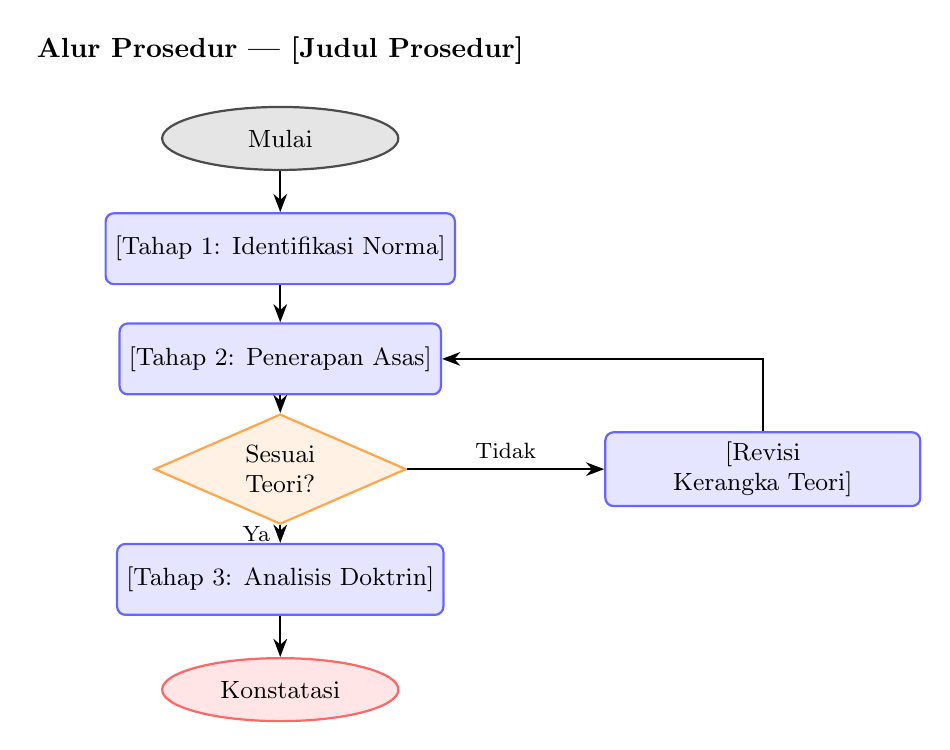
\begin{tikzpicture}[
  node distance=1.4cm,
  every node/.style={font=\small},
  start/.style={
    ellipse, draw=black!70, thick, fill=gray!20,
    minimum width=3cm, minimum height=0.8cm, align=center
  },
  proses/.style={
    rectangle, draw=blue!60, thick, fill=blue!10,
    minimum width=4cm, minimum height=0.9cm,
    rounded corners=3pt, align=center
  },
  keputusan/.style={
    diamond, draw=orange!70, thick, fill=orange!10,
    minimum width=3.2cm, minimum height=0.9cm,
    aspect=2, align=center
  },
  akhir/.style={
    ellipse, draw=red!60, thick, fill=red!10,
    minimum width=3cm, minimum height=0.8cm, align=center
  },
  arrow/.style={-Stealth, thick}
]

\node[start]     (mulai)   {Mulai};
\node[proses]    (p1)      [below of=mulai]   {[Tahap 1: Identifikasi Norma]};
\node[proses]    (p2)      [below of=p1]      {[Tahap 2: Penerapan Asas]};
\node[keputusan] (k1)      [below of=p2]      {Sesuai\\Teori?};
\node[proses]    (p3ya)    [below of=k1]      {[Tahap 3: Analisis Doktrin]};
\node[proses]    (p3tidak) [right=2.5cm of k1]{[Revisi\\Kerangka Teori]};
\node[akhir]     (selesai) [below of=p3ya]    {Konstatasi};

\draw[arrow] (mulai)   -- (p1);
\draw[arrow] (p1)      -- (p2);
\draw[arrow] (p2)      -- (k1);
\draw[arrow] (k1)      -- node[left]{\footnotesize Ya}  (p3ya);
\draw[arrow] (k1)      -- node[above]{\footnotesize Tidak} (p3tidak);
\draw[arrow] (p3tidak) |- (p2);
\draw[arrow] (p3ya)    -- (selesai);

\node[above=0.4cm of mulai, font=\bfseries]
  {Alur Prosedur — [Judul Prosedur]};

\end{tikzpicture}

\end{document}
 ke artikel Anda
%============================================================

\documentclass[tikz,border=10pt]{standalone}
\usepackage{tikz}
\usetikzlibrary{shapes.geometric, arrows.meta, positioning, fit, backgrounds, shadows}

\begin{document}

%------------------------------------------------------------
%  DIAGRAM 1: Kerangka ATD — Analisis Kasus
%------------------------------------------------------------
\begin{tikzpicture}[
  node distance = 1.6cm,
  every node/.style = {font=\small},
  box/.style = {
    rectangle, rounded corners=4pt, minimum width=3.8cm, minimum height=1cm,
    align=center, draw, thick
  },
  norma/.style   = {box, fill=blue!15,   draw=blue!60},
  asas/.style    = {box, fill=green!15,  draw=green!60},
  teori/.style   = {box, fill=orange!15, draw=orange!60},
  doktrin/.style = {box, fill=purple!15, draw=purple!60},
  hasil/.style   = {
    rectangle, rounded corners=6pt, minimum width=8cm, minimum height=1.2cm,
    align=center, draw=red!70, thick, fill=red!10
  },
  arrow/.style   = {-Stealth, thick, gray}
]

% Baris atas: empat elemen ATD
\node[norma]   (N) {Norma Positif\\{\footnotesize (Pasal/UU/Putusan)}};
\node[asas]    (A) [right=1.2cm of N] {Asas Hukum\\{\footnotesize (Ratio Legis)}};
\node[teori]   (T) [right=1.2cm of A] {Teori Hukum\\{\footnotesize (Filosofis/Yuridis)}};
\node[doktrin] (D) [right=1.2cm of T] {Doktrin Hukum\\{\footnotesize (Pendapat Ahli)}};

% Simbol plus di antara node
\node at ($(N.east)!0.5!(A.west)$) {\textbf{+}};
\node at ($(A.east)!0.5!(T.west)$) {\textbf{+}};
\node at ($(T.east)!0.5!(D.west)$) {\textbf{+}};

% Kotak hasil di bawah
\node[hasil] (H) [below=2cm of $(N.south)!0.5!(D.south)$]
  {\textbf{Konstatasi / Analisis Kasus}\\
   {\footnotesize [Isi dengan temuan analisis hukum Anda]}};

% Panah dari masing-masing elemen ke hasil
\draw[arrow] (N.south) -- ++(0,-0.6) -| (H.north);
\draw[arrow] (A.south) -- ++(0,-0.6) -| (H.north);
\draw[arrow] (T.south) -- ++(0,-0.6) -| (H.north);
\draw[arrow] (D.south) -- ++(0,-0.6) -| (H.north);

% Label judul
\node[above=0.4cm of $(N.north)!0.5!(D.north)$, font=\bfseries]
  {Kerangka Analisis ATD — LEX v3.0};

\end{tikzpicture}

%------------------------------------------------------------
%  DIAGRAM 2: Alur Prosedur Hukum (Flowchart)
%  Ganti label sesuai prosedur yang Anda analisis
%------------------------------------------------------------
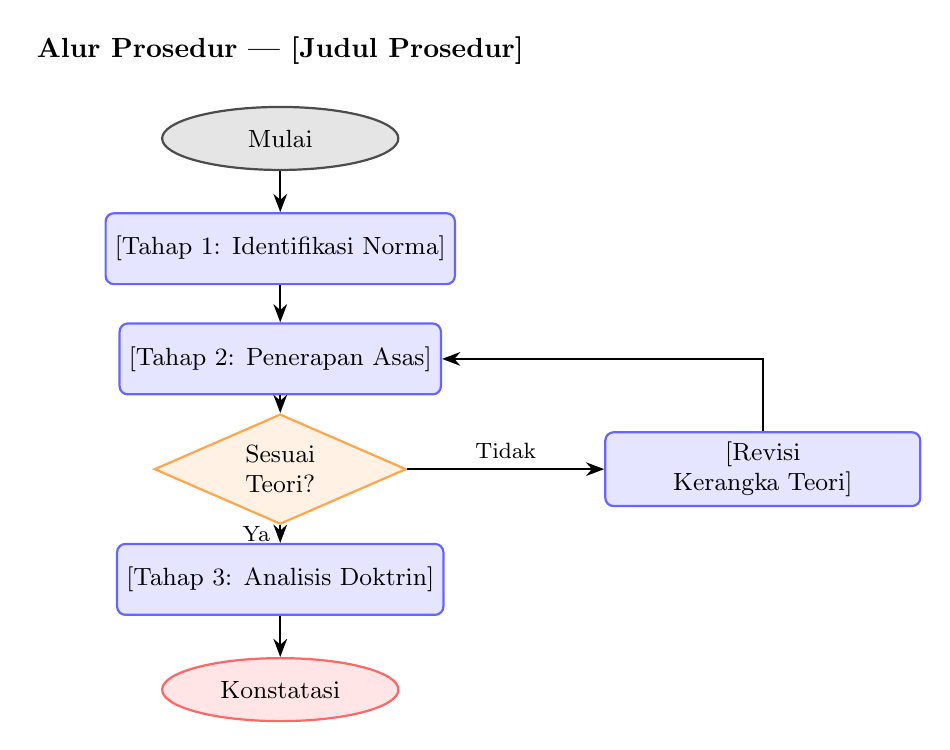
\begin{tikzpicture}[
  node distance=1.4cm,
  every node/.style={font=\small},
  start/.style={
    ellipse, draw=black!70, thick, fill=gray!20,
    minimum width=3cm, minimum height=0.8cm, align=center
  },
  proses/.style={
    rectangle, draw=blue!60, thick, fill=blue!10,
    minimum width=4cm, minimum height=0.9cm,
    rounded corners=3pt, align=center
  },
  keputusan/.style={
    diamond, draw=orange!70, thick, fill=orange!10,
    minimum width=3.2cm, minimum height=0.9cm,
    aspect=2, align=center
  },
  akhir/.style={
    ellipse, draw=red!60, thick, fill=red!10,
    minimum width=3cm, minimum height=0.8cm, align=center
  },
  arrow/.style={-Stealth, thick}
]

\node[start]     (mulai)   {Mulai};
\node[proses]    (p1)      [below of=mulai]   {[Tahap 1: Identifikasi Norma]};
\node[proses]    (p2)      [below of=p1]      {[Tahap 2: Penerapan Asas]};
\node[keputusan] (k1)      [below of=p2]      {Sesuai\\Teori?};
\node[proses]    (p3ya)    [below of=k1]      {[Tahap 3: Analisis Doktrin]};
\node[proses]    (p3tidak) [right=2.5cm of k1]{[Revisi\\Kerangka Teori]};
\node[akhir]     (selesai) [below of=p3ya]    {Konstatasi};

\draw[arrow] (mulai)   -- (p1);
\draw[arrow] (p1)      -- (p2);
\draw[arrow] (p2)      -- (k1);
\draw[arrow] (k1)      -- node[left]{\footnotesize Ya}  (p3ya);
\draw[arrow] (k1)      -- node[above]{\footnotesize Tidak} (p3tidak);
\draw[arrow] (p3tidak) |- (p2);
\draw[arrow] (p3ya)    -- (selesai);

\node[above=0.4cm of mulai, font=\bfseries]
  {Alur Prosedur — [Judul Prosedur]};

\end{tikzpicture}

\end{document}
 ke artikel Anda
%============================================================

\documentclass[tikz,border=10pt]{standalone}
\usepackage{tikz}
\usetikzlibrary{shapes.geometric, arrows.meta, positioning, fit, backgrounds, shadows}

\begin{document}

%------------------------------------------------------------
%  DIAGRAM 1: Kerangka ATD — Analisis Kasus
%------------------------------------------------------------
\begin{tikzpicture}[
  node distance = 1.6cm,
  every node/.style = {font=\small},
  box/.style = {
    rectangle, rounded corners=4pt, minimum width=3.8cm, minimum height=1cm,
    align=center, draw, thick
  },
  norma/.style   = {box, fill=blue!15,   draw=blue!60},
  asas/.style    = {box, fill=green!15,  draw=green!60},
  teori/.style   = {box, fill=orange!15, draw=orange!60},
  doktrin/.style = {box, fill=purple!15, draw=purple!60},
  hasil/.style   = {
    rectangle, rounded corners=6pt, minimum width=8cm, minimum height=1.2cm,
    align=center, draw=red!70, thick, fill=red!10
  },
  arrow/.style   = {-Stealth, thick, gray}
]

% Baris atas: empat elemen ATD
\node[norma]   (N) {Norma Positif\\{\footnotesize (Pasal/UU/Putusan)}};
\node[asas]    (A) [right=1.2cm of N] {Asas Hukum\\{\footnotesize (Ratio Legis)}};
\node[teori]   (T) [right=1.2cm of A] {Teori Hukum\\{\footnotesize (Filosofis/Yuridis)}};
\node[doktrin] (D) [right=1.2cm of T] {Doktrin Hukum\\{\footnotesize (Pendapat Ahli)}};

% Simbol plus di antara node
\node at ($(N.east)!0.5!(A.west)$) {\textbf{+}};
\node at ($(A.east)!0.5!(T.west)$) {\textbf{+}};
\node at ($(T.east)!0.5!(D.west)$) {\textbf{+}};

% Kotak hasil di bawah
\node[hasil] (H) [below=2cm of $(N.south)!0.5!(D.south)$]
  {\textbf{Konstatasi / Analisis Kasus}\\
   {\footnotesize [Isi dengan temuan analisis hukum Anda]}};

% Panah dari masing-masing elemen ke hasil
\draw[arrow] (N.south) -- ++(0,-0.6) -| (H.north);
\draw[arrow] (A.south) -- ++(0,-0.6) -| (H.north);
\draw[arrow] (T.south) -- ++(0,-0.6) -| (H.north);
\draw[arrow] (D.south) -- ++(0,-0.6) -| (H.north);

% Label judul
\node[above=0.4cm of $(N.north)!0.5!(D.north)$, font=\bfseries]
  {Kerangka Analisis ATD — LEX v3.0};

\end{tikzpicture}

%------------------------------------------------------------
%  DIAGRAM 2: Alur Prosedur Hukum (Flowchart)
%  Ganti label sesuai prosedur yang Anda analisis
%------------------------------------------------------------
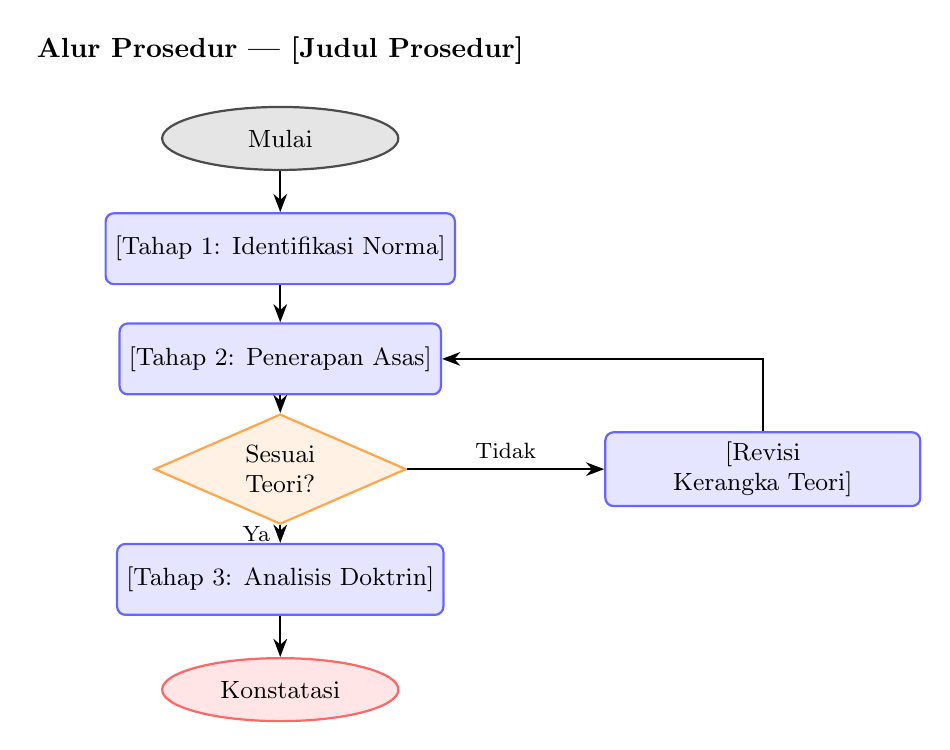
\begin{tikzpicture}[
  node distance=1.4cm,
  every node/.style={font=\small},
  start/.style={
    ellipse, draw=black!70, thick, fill=gray!20,
    minimum width=3cm, minimum height=0.8cm, align=center
  },
  proses/.style={
    rectangle, draw=blue!60, thick, fill=blue!10,
    minimum width=4cm, minimum height=0.9cm,
    rounded corners=3pt, align=center
  },
  keputusan/.style={
    diamond, draw=orange!70, thick, fill=orange!10,
    minimum width=3.2cm, minimum height=0.9cm,
    aspect=2, align=center
  },
  akhir/.style={
    ellipse, draw=red!60, thick, fill=red!10,
    minimum width=3cm, minimum height=0.8cm, align=center
  },
  arrow/.style={-Stealth, thick}
]

\node[start]     (mulai)   {Mulai};
\node[proses]    (p1)      [below of=mulai]   {[Tahap 1: Identifikasi Norma]};
\node[proses]    (p2)      [below of=p1]      {[Tahap 2: Penerapan Asas]};
\node[keputusan] (k1)      [below of=p2]      {Sesuai\\Teori?};
\node[proses]    (p3ya)    [below of=k1]      {[Tahap 3: Analisis Doktrin]};
\node[proses]    (p3tidak) [right=2.5cm of k1]{[Revisi\\Kerangka Teori]};
\node[akhir]     (selesai) [below of=p3ya]    {Konstatasi};

\draw[arrow] (mulai)   -- (p1);
\draw[arrow] (p1)      -- (p2);
\draw[arrow] (p2)      -- (k1);
\draw[arrow] (k1)      -- node[left]{\footnotesize Ya}  (p3ya);
\draw[arrow] (k1)      -- node[above]{\footnotesize Tidak} (p3tidak);
\draw[arrow] (p3tidak) |- (p2);
\draw[arrow] (p3ya)    -- (selesai);

\node[above=0.4cm of mulai, font=\bfseries]
  {Alur Prosedur — [Judul Prosedur]};

\end{tikzpicture}

\end{document}
